\documentclass[11pt,a4paper]{article}
\usepackage[utf8]{inputenc}
\usepackage{graphicx}


\textheight=22cm
\textwidth=14.945cm
\topmargin=0.5cm
\headheight=0cm
\headsep=0cm
\oddsidemargin=0.5cm
\evensidemargin=0.5cm
\columnsep=0.8cm
\renewcommand{\baselinestretch}{1.3}

\begin{document}

\begin{titlepage}
  \begin{center} \sloppy
    \large \textsc{Project YaJTris - Yet another Java Tetris clone }
    \vfill

    \huge \textbf{Functional Specifications} \vfill 

    \LARGE Jussi Mäki - joamaki@gmail.com
    \vspace{3mm}
    
    A programming project\\
    for Mika Holmström, University of Helsinki, Computer Science department

    \vfill

    Helsinki \today
    % \number\day .\number\month .\number\year

  \end{center}
\end{titlepage}

\section {Introduction}

This document describes the functional specifications of YaJTris in regards to 
purpose, appearance and behaviour.

The implementation details are outside the scope of this document and are described in the 
implementation plan.

\section {Purpose and overview}

{\bf YaJTris} is a clone of the popular single-player game Tetris by Alexey Pajitnov. 
The goal in the game is to rotate and move tetrominoes (7 individual pieces composed of 4 squares in different configurations) that fall from above so that they fall down to form 
horizontal lines without gaps. When a line forms it disappears and any blocks above it 
will fall to fill the gap. As the game progresses the tetrominoes will fall faster and
faster. When the stack of tetrominoes reaches the top of the area the game ends. 

\vspace{3mm}
The seven tetriminoes (not necessarely as they appear in the final product):
\begin{center}
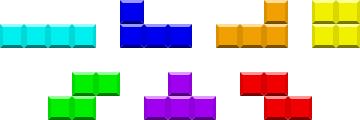
\includegraphics{tetrominoes.png}
\end{center}

\section {Restrictions}

The game area is restricted to an area of 10 blocks wide and 20 blocks high. No restrictions
are made to the maximum speed of tetriminoes. The maximum score is also unrestricted but
implementation can use an overflowable data type that fits an humanly attainable score.

The size of the application window is restricted by the size of the game area and shall
not support resizing.

High scores are limited to 10 entries.

Player's name in high scores is limited to 9 characters from A-Z.

\section {Data flow}

Tetriminoes are rotated by using the cursor keys. The program allows rotation 
of the piece when the rotation does not result in a collision with the walls of the game
area or with another piece. Tetrimino can be moved around the screen left and right. The
user can also speed up the falling pace of the square. A collision to the vertical sides
of the square shall restrict the movement of the square sideways. When the square collides
at the bottom it shall become static and if it filled a row of squares the row disappears.

The program loads and saves high score data in a file. File shall contain
the player's name and score.

\section {Functionality and behaviour}

The game consists of the area of tetriminoes, a box showing the next tetrimino, the current
score, list of instructions and a list of top 10 highest scores. 
The player has control over the current tetromino's rotation and horizontal position using cursor keys. The {\bf Left} and
{\bf Right} cursor keys move the piece left and right respectively. The {\bf Up} key rotates the piece. The {\bf Down} key makes the piece drop faster. To completely drop a piece player can press the '{\bf Space}' key. For each piece dropped the player is awarded 10 points.

To exit the game player can press the '{\bf Escape}' key. The program shall verify that the
user really wants to exit the game in case the user mispressed the key.

When the game ends and the player reaches a top 10 high score the game shall ask the player for a name.

\vspace{3mm}
Mockup of YaJTris:
\begin{center}
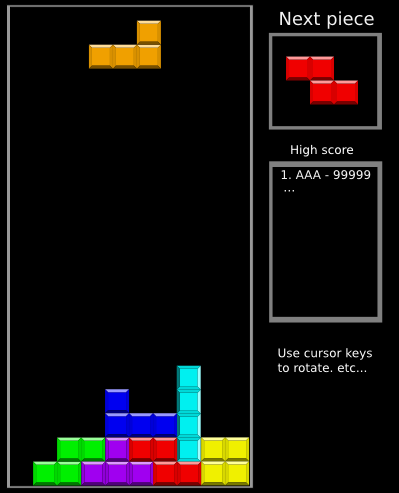
\includegraphics[scale=0.5]{tetris_mockup.png}
\end{center}

\end{document}